\documentclass[titlepage,12pt]{article}
\usepackage[utf8]{inputenc}
\usepackage {mathtools, graphicx, amsfonts, amssymb, comment}
\usepackage{enumerate}
\usepackage{geometry}
\usepackage{subcaption}
\usepackage{float}
\usepackage[backend=bibtex,sorting=none]{biblatex}
\usepackage{listings}
\usepackage{hyperref}

% http://tex.stackexchange.com/questions/118173/how-to-write-ceil-and-floor-in-latex
\DeclarePairedDelimiter\ceil{\lceil}{\rceil}
\DeclarePairedDelimiter\floor{\lfloor}{\rfloor}

% Declare sgn function
\DeclareMathOperator{\sgn}{sgn}

\addbibresource{bibliography.bib}
\geometry{margin=1.25in}

% http://tex.stackexchange.com/questions/65849/confusion-onehalfspacing-vs-spacing-vs-word-vs-the-world
\linespread{1.25}

\title{The JPEG 2000}
\author{Matt Gaikema \\ Will Argueta}
\date{May 2016}

\begin{document}

\maketitle

%%%%%%%%%%%%%%%%
% INTRODUCTION %
%%%%%%%%%%%%%%%%
\section{Introduction}

In order to efficiently send and receive images, it is often useful to compress them, 
since much of the data may be irrelevant or redundant.
One of the many ways of accomplishing this is through wavelets.

There are two types of image compression: lossy and lossless.
\textbf{Lossless} compression means that every bit of information is recovered from the compressed data,
while \textbf{lossy} compression occurs when redundant information is eliminated.
The GIF is an example of lossless compression, while the JPEG is lossy.

The JPEG 2000 is one method of image compression which uses wavelets.
It was created in 2000 by the Joint Photographic Experts Group with the aim of replacing the original JPEG standard, 
which uses the Discrete Cosine Transform and was created in 1992.
The file extension is \verb|.jp2|, compared with the typical JPEG extension of \verb|.jpg|.

% http://www.verypdf.com/pdfinfoeditor/jpeg-jpeg-2000-comparison.htm
\begin{figure}[h]
	\centering
	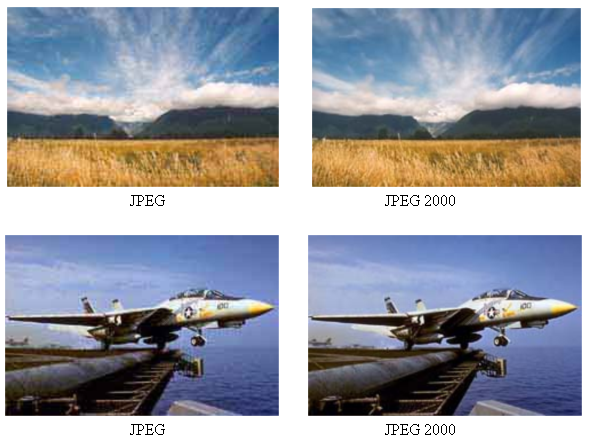
\includegraphics[scale=0.4]{resources/comparison.png}
	\caption{Two images compressed using JPEG and JPEG 2000.\cite{comparison}}
	\label{fig:compare}
\end{figure}

There are a few advantages of the JPEG 2000 over the JPEG,
thanks to the JPEG 2000's use of wavelets.
First, JPEG 2000 can be lossy or lossless, while JPEG compression is always lossy.
This means that JPEG 2000 produces images of much higher quality.
Figure \ref{fig:compare} shows two images compressed both using JPEG and JPEG 2000.

Of course, despite the advantages of the JPEG 2000, it is rarely used today, 
while the JPEG is still very popular.
The main reason is computation.\cite{alternative} 
Adopting the JPEG 2000 would have required rewriting much software, 
since it was not backwards-compatable with the JPEG.
Many companies were unwilling to add support for it since it wasn't popular,
and many consumers didn't use it since there was little support for it,
creating an unfortunate cycle. 
Additionally, the JPEG 2000 requires more computing power, which was not as abundant in 2000 as it is today.
To this day, few websites and no major web browsers support it.


%%%%%%%%%%%%%%%%%%%%%%%%%%%
% MATHEMATICAL BACKGROUND %
%%%%%%%%%%%%%%%%%%%%%%%%%%%
\section{Mathematical Background}
% https://en.wikipedia.org/wiki/JPEG_2000

The JPEG 2000's use of the Discrete Wavelet Transform is what makes it superior to the JPEG.\cite{how}
The Discrete Cosine Transform (DCT), which is used by the JPEG, compresses the image into 8x8 blocks
and places them consecutively in the file.
The blocks are compressed individually.
This is the reason for "blockiness" in compressed JPEG images.

Wavelet compression converts the image into a series of wavelets, which can be more easily stored than pixel blocks.

The JPEG 2000 compression algorithm consists of four basic steps: 
preprocess, transformation, quantization, and encoding\cite{whydomath}.

% A lossy transform on the baby picture.
\begin{figure}[h]
	\centering
	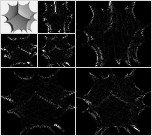
\includegraphics[scale=0.6]{resources/lossybaby.png}
	\caption{DWT coefficients using the lossy 9/7 filter.}
	\label{fig:lossybaby}
\end{figure}

% A lossless transform on the baby picture.
\begin{figure}[h]
	\centering
	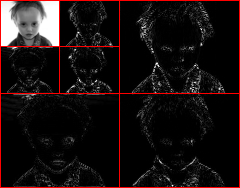
\includegraphics[scale=0.6]{resources/losslessbaby.png}
	\caption{DWT coefficients using the lossless 5/3 filter.}
	\label{fig:losslessbaby}
\end{figure}

\begin{enumerate}
	
	% PREPROCESSING %
	\item\textbf{Preprocecessing:}
	If the image is a color image, the image needs to be converted to the YCbCr color space\cite{colorspace}
	from the standard RGB color space.

	After the color space transform, sometimes the image will be split up into different tiles of equal size,
	but this is optional.
	
	% TRANSFORM %
	\item\textbf{Transform:}
	The Discrete Wavelet Transform is the most impportant feature of the JPEG 2000.
	In the case of a lossy compression, a Cohen-Daubechies-Feauveau (CDF) 9/7 wavelet is used,
	while the CDF 5/3 wavelet is used for lossless compression.
	In both cases, between two and three iterations are computed, using the lifting method.
	
	% QUANTIZATION %
	\item\textbf{Quantization:}
	Quantization refers to the process of compressing a range of values into a single value,
	and is used in lossy compression.
	Quantization is usually the main source of error in compression.\cite{clifford}
	If the compression is lossless, then no quantization is done.
	Figure \ref{fig:losslessbaby} is encoded and the algorithm is completed.
	
	In a lossy compression, more work must be done.
	The quantization scheme used is not unlike that used by JPEG on the 8x8 blocks,
	where two iterations of the DWT results in seven blocks.
	A floor function is applied to each of the wavelet coefficients.
	The function used for quantization is
	\begin{equation}
		q(t) = \sgn(t)\floor*{|t|/d},
	\end{equation}
	where $d$ is the step size.\cite{whydomath}
	For a lossless compression, $d=1$.
	For a lossy compression, a different step size is used for each level,
	using the base step size, which is defined as
	\begin{equation}
		\tau = 2^{R+i-c}(1+f/2^{11}).
	\end{equation}
	$R$ is the number of bits required to represent the original intensities,
	$i$ is the number of levels of the Discrete Wavelet Transform,
	and $c$ and $f$ are used in blurring.
	The step size at each level is $d=\tau/2^i$.
	
	% ENCODING %
	\item\textbf{Encoding:}
	For encoding, Embedded Block Coding with Optimized Truncation, or EBCOT, is used,
	which is another difference the JPEG 2000 has from JPEG, 
	which uses Huffman Coding.
	The EBCOT algorithm is used to code the wavelet coefficients.
	
	The EBCOT algorithm uses subband coding.
	The result of the quantization step is a set of subbands, 
	where a subband is a collection of real coefficients representing a certain
	frequency range and region of the image.
	
	Each subband is split into different blocks,
	and each block is then coded independently.\cite{hp}
	For more information on the EBCOT method of coding, 
	see \cite{ebcot}.
	
\end{enumerate}

\begin{figure}[h]
	\centering
	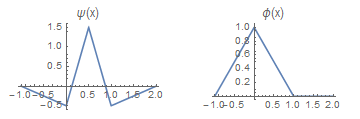
\includegraphics[scale=0.9]{resources/lossless_family.png}
	\caption{Wavelet and scaling functions for the CDF 5/3 transform.}
	\label{fig:lossless_family}
\end{figure}

\begin{figure}[h]
	\centering
	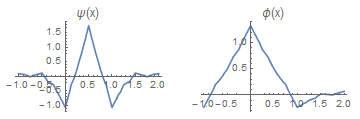
\includegraphics[scale=0.9]{resources/lossy_family.png}
	\caption{Wavelet and scaling functions for the CDF 9/7 transform.}
	\label{fig:lossy_family}
\end{figure}

\subsection{The CDF Wavelet}
% http://www.ams.org/samplings/feature-column/fcarc-image-compression

The CDF Wavelet is a biorthogonal wavelet, which, in addition to satisfying the requirements for a multiresolution analysis,
satisfies four properties\cite{old}:
\begin{itemize}
	\item The scaling function, $\phi(x)$, is always symmetric.
	\item The wavelet function, $\psi(x)$, is always symmetric or anti-symmetric.
	\item The wavelet filters are finite.
	\item The coefficients of the wavelet filters have the form $\frac{z}{2^n}$, with $z\in\mathbb{Z}$ and $n\in\mathbb{N}$.
\end{itemize}
Figures \ref{fig:lossy_family} and \ref{fig:lossless_family} show plots of the $\phi(x)$
and $\psi(x)$ for the lossy and lossless transforms, respectively.

Similar to the Daubechies Wavelet, the CDF wavelet is constructed using a polynomial.
For every positive integer $A$ there is a unique polynomial $Q_A(x)$ of degree $A-1$ such that
\[(1-\frac{x}{2})^AQ_A(x)+(\frac{x}{2})^AQ_A(2-x)=1,\]
where $Q_A$ is factored so that
\[Q_A(x)=q_{prim}(x)q_{dual}(x).\]
$q_{prim}$ and $q_{dual}$ are polynomials with real coefficients and a constant coefficient of 1.
Then,
\begin{align*}
	a_{prim}(z) =& 2z^d(\frac{1+z}{2})^Aq_{prim}(1-\frac{z+z^{-1}}{2}) \\
	a_{dual}(z) =& 2z^d(\frac{1+z}{2})^Aq_{dual}(1-\frac{z+z^{-1}}{2})
\end{align*}
are a pair of biorthogonal scaling sequences.
Here, $d$ is an arbitrary integer used to center the sequences and make the filters causal.

Since the CDF wavelet is biorthogonal, there are two wavelet bases, $\psi_{mn}$ and $\tilde{\psi}_{mn}$,
which are shifts and scalings of $\psi$ and $\tilde{\psi}$.\cite{cdf}
For any $f\in L^2(\mathbb{R})$, we have that
\begin{equation}
	f = \sum_{j,k\in\mathbb{Z}}\langle f,\tilde{\psi}_{jk}\rangle\psi_{jk}=\sum_{j,k\in\mathbb{Z}}\langle f,\psi_{jk}\rangle\tilde{\psi}_{jk}.
\end{equation}
The two scaling functions $\phi(x)$ and $\tilde{\phi}(x)$ are referred to 
as the primal and dual scaling functions, respectively.\cite{cdfwhat}
As usual, dilations and translations of a function $g(x)$ are defined by 
\[g_{j,k}(x)=2^{j/2}g(2^jx-k).\]

%\bigskip
%\noindent
%The wavelet transform on an image produces as many coefficients as there are pixels.

\begin{figure}
	\centering
	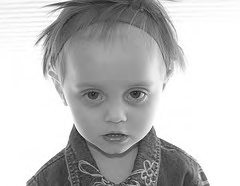
\includegraphics{resources/baby.png}
	\caption{An untransformed grayscale image.}
	\label{fig:original}
\end{figure}


%%%%%%%%%%%%%%%
% APPLICATION %
%%%%%%%%%%%%%%%
\section{Application}

The source code for the implemented transformations in Mathematica can be found at \cite{implement}.
Figure \ref{fig:original} is the image, untransformed and uncompressed.
Since it is a grayscale image, no color space conversions needs to be done.
Figures \ref{fig:lossybaby} and \ref{fig:losslessbaby} show the results of a lossy and lossless 
discrete wavelet transforms, respectively.

\begin{figure}
	\centering
	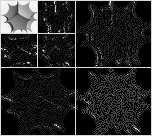
\includegraphics{resources/quantBabyPlot.png}
	\caption{The result of quantization on the 9/7 wavelet coefficients.}
	\label{fig:quantBabyPlot}
\end{figure}

The next step is quantization.
For the lossless compression, this step is skipped.
For the lossy compression, the quantiation function
\[q(t)=\frac{\floor{t*16}}{16}\]
was applied to each coefficient for simplicity.
Figure \ref{fig:quantBabyPlot} shows the result of quantization on the 9/7 wavelet coefficients.

\begin{figure}
	\centering
	
\includegraphics{resources/finalLossyBaby.png}
	\caption{The compressed image, after a lossy compression.}
	\label{fig:finalLossyBaby}
\end{figure}
\begin{figure}
	\centering
	
\includegraphics{resources/finalLosslessBaby.png}
	\caption{The compressed image, after a lossless compression.}
	\label{fig:finalLosslessBaby}
\end{figure}

The final step is encoding.
The EBCOT algorithm is automatically performed by Mathematica 
when performing a JPEG 2000 compression.
Figures \ref{fig:finalLossyBaby} and \ref{fig:finalLosslessBaby} 
show the final results of lossy and lossless compressions, respectively.

\begin{figure}[p]
	\centering
	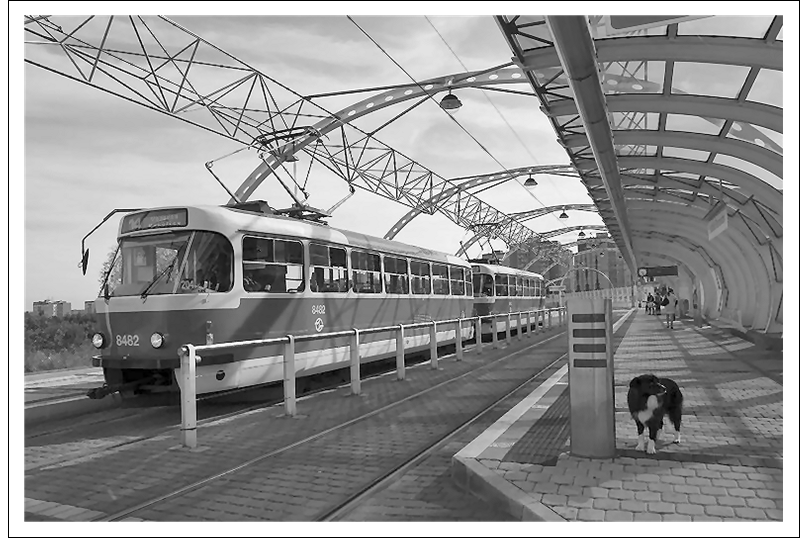
\includegraphics[scale=0.35]{resources/example/originalExample.png}
	\caption{An untransformed image.}
	\label{fig:originalExample}
\end{figure}
\begin{figure}
    \centering
    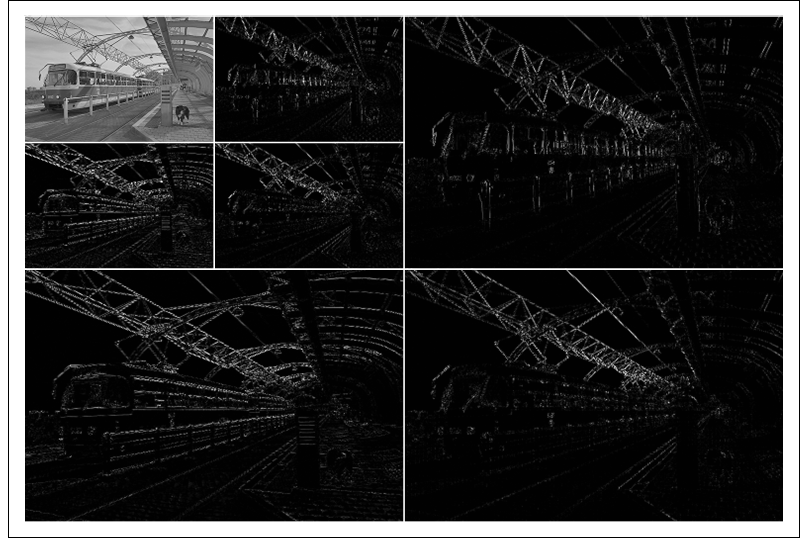
\includegraphics[scale=0.35]{resources/example/losslessTransform.png}
    \caption{The result of the CDF 5/3 wavelet transform.}
    \label{fig:losslessTransform}
\end{figure}
\begin{figure}
    \centering
    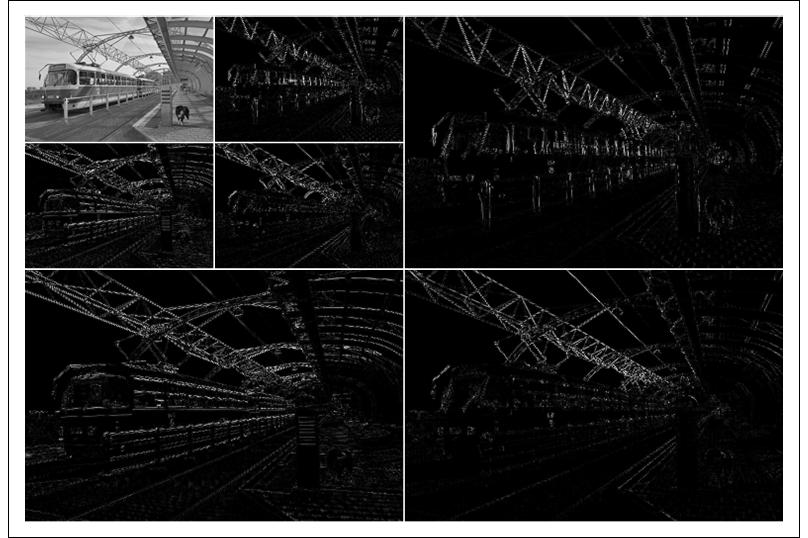
\includegraphics[scale=0.35]{resources/example/lossyTransform.png}
    \caption{The result of a CDF 9/7 wavelet transform.}
    \label{fig:lossyTransform}
\end{figure}
\begin{figure}
	\centering
	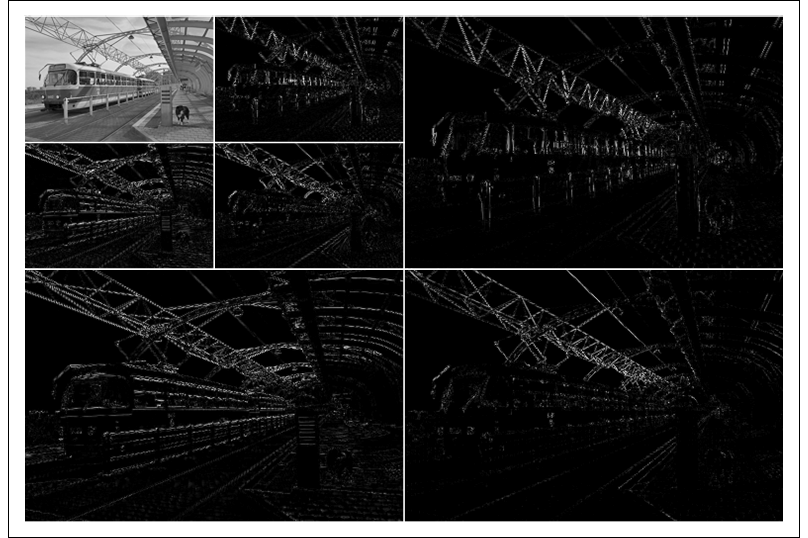
\includegraphics[scale=0.35]{resources/example/exampleQuant.png}
	\caption{The result of quantizing the coefficients of the 9/7 DWT.}
	\label{fig:exampleQuant}
\end{figure}
\begin{figure}
	\centering
	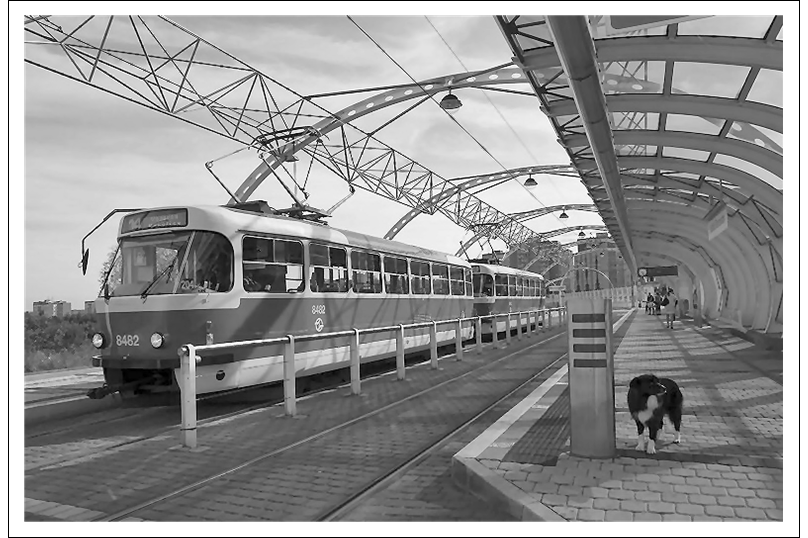
\includegraphics[scale=0.35]{resources/example/exampleCompressed.png}
	\caption{The compressed image, using lossy techniques.}
	\label{fig:exampleCompressed}
\end{figure}

A more complete example can be found at \cite{whydomath}.
Figure \ref{fig:originalExample} shows the original, uncompressed image.
Figure \ref{fig:losslessTransform} shows the result of a CDF 5/3 wavelet transform,
and Figure \ref{fig:lossyTransform} shows the result of a CDF 9/7 wavelet transform.
The quantized coefficients of the CDF 9/7 DWT are shown in Figure \ref{fig:exampleQuant}.
The compressed image is shown in Figure \ref{fig:exampleCompressed}, 
and can be compared with Figure \ref{fig:originalExample}.


%%%%%%%%%%%%%%
% CONCLUSION %
%%%%%%%%%%%%%%
\section{Conclusion}

The JPEG 2000 could easily be the next standard for image compression, if only people would use it.
It uses much more sophisticated techniques than the JPEG to improve image quality and compression,
but computational requirements made it unattractive.
For performing a lossless compression, the PNG is more efficient, space-wise and computationally.

The JPEG 2000 is best-suited for large images and images with low-contrast edges,
which are primarily medical images.
In fact, this was one of the primary intended purposes of the JPEG 2000.
Digital Imaging and Communications in Medicine (DICOM), 
which is the international standard for medical imaging.\cite{dicom}

We demonstrated the superiority of image quality after a JPEG 2000 compression, 
and its ability to perform both lossy and lossless compression gives it a 
great degree of versatility, which the JPEG lacks.


%%%%%%%%%%%%%%
% REFERENCES %
%%%%%%%%%%%%%%
\printbibliography


%\clearpage
%\lstinputlisting{main.wl}

\end{document}
